\documentclass[tikz]{standalone}
\usepackage{amsmath} \\ \DeclareFontFamily{U}{skulls}{} \\ \DeclareFontShape{U}{skulls}{m}{n}{ <-> skull }{} \\ \newcommand{\skull}{\text{\usefont{U}{skulls}{m}{n}\symbol{'101}}}
\begin{document}
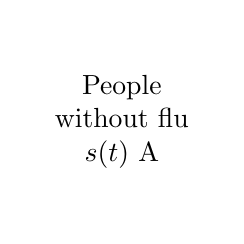
\begin{tikzpicture}[]
  \def\Radius{1cm}
  %\draw  (0cm,0cm) circle[radius=\Radius] node {People without flu $s(t)$};
  \node[circle, align = center] { People \\ without flu \\ $s(t)$ $\skull$};

\end{tikzpicture}

\end{document}
